% !TEX TS-program = lualatex
% !TEX encoding = UTF-8

\documentclass[Session2026.tex]{subfiles}

\ifcsname preamble@file\endcsname
  \setcounter{page}{\getpagerefnumber{M-07_samedi}}
\fi

\begin{document}

\addcontentsline{toc}{chapter}{Samedi 11 juillet, saint Benoît}

\bigtitle{Saint Benoît, à la Messe}{samedi 11 juillet}{Messe}

\gscore{in_gaudeamus_benedicti}
\translation{\aa Réjouissons-nous tous dans le Seigneur, le jour où nous célébrons la fête en l'honneur de Benoît, abbé : la solennité dont se réjouissent les anges, ensemble, ils louent le Fils de Dieu.\\
\vv Le Seigneur est grand, il est l'objet de toute louange, dans la cité de notre Dieu.}

\newpage

\vspace*{2cm}

\smalltitle{Psalmodie de Tierce}

\gscore{an_beatus_vir_ps119}
\translation{\aa Le bienheureux Benoît désira davantage de souffrir les maux du monde que d'en recevoir les louanges, de s'épuiser en travaux pour Dieu que d'être flatté par les plaisirs de cette vie.}
\smalltitle{Psaume 119}
\psalm{119}{3}
\smalltitle{Psaume 120}
\psalm{120}{3}
\needspace{3cm}
\smalltitle{Psaume 121}
\psalm{121}{3}

\smalltitle{Kyrie II}
\gscore{ky_k2}

\smalltitle{Gloria II}
\gscore{ky_g2}

\gscore{gr_domine_praevenisti}
\translation{\rr Seigneur, tu l'as prévenu des plus douces bénédictions; Tu as mis sur sa tête une couronne de pierres précieuses.\\
\vv Il t'a demandé la vie, et tu lui as accordé des jours qui dureront dans les siècles des siècles.}

\gscore{al_vir_dei_benedictus}
\translation{\vv L'homme de Dieu Benoît était rempli de l'esprit de tous les saints : il intercède pour tous ceux qui ont fait profession monastique.}

\gscore{se_laeta_dies}
\translation{\colored{C}ette journée qui resplendit d’un éclat nouveau, est celle où notre grand chef entra dans son repos.\\
\colored{L}a grâce a visite l’âme filiale de ses enfants ; que leurs chants soient dignes de l’amour qui enflamme leurs cœurs.\\
\colored{A}dmirons notre Patriarche qui s’élève par un chemin céleste, à l’orient.\\
\colored{L}’innombrable famille sortie de lui l’a fait l’égal d’Abraham semblable au soleil.\\
\colored{C}’est Elie caché au fond de son antre ; un corbeau exécute ses ordres.\\
\colored{C}’est Elisée, quand il retire la hache tombée au fond du lac.\\
\colored{P}ar la pureté de sa vie il ressemble à Joseph; par son esprit prophétique il retrace Jacob.\\
\colored{Q}u’il daigne se souvenir des enfants dont il est le Père, et qu’il nous conduise aux joies éternelles du Christ qui demeure à jamais ! Amen.
}

\newpage

\smalltitle{Credo IV}
\gscore{ky_c4}

\pagebreak

\gscore{of_desiderium_animae}
\translation{\rr Tu lui as accordé le désir de son cœur, et tu ne l'as pas frustré de la demande de ses lèvres. Tu as mis sur sa tête une couronne de pierres précieuses.}

\smalltitle{Sanctus II}
\gscore{ky_s2}

\pagebreak

\smalltitle{Agnus II}
\gscore{ky_a2}

\newpage

\gscore{co_semel_juravi}
\translation{\aa Je l'ai jadis juré par moi-même, et je ne mentirai pas à David: sa race demeurera éternellement, et son trône sera comme le soleil en ma présence, et comme la lune qui subsistera à jamais, et le témoin qui est au ciel est fidèle.}

\smalltitle{Ite II}
\gscore{ky_i2}

{\footnotesize\hfill\rubric{Ci-contre: le roi David, stalles de l'abbaye de Solesmes, \copyright{} Jacques Baguenier}}
\newpage

\newgeometry{scale=1, headsep=0mm}%
\noindent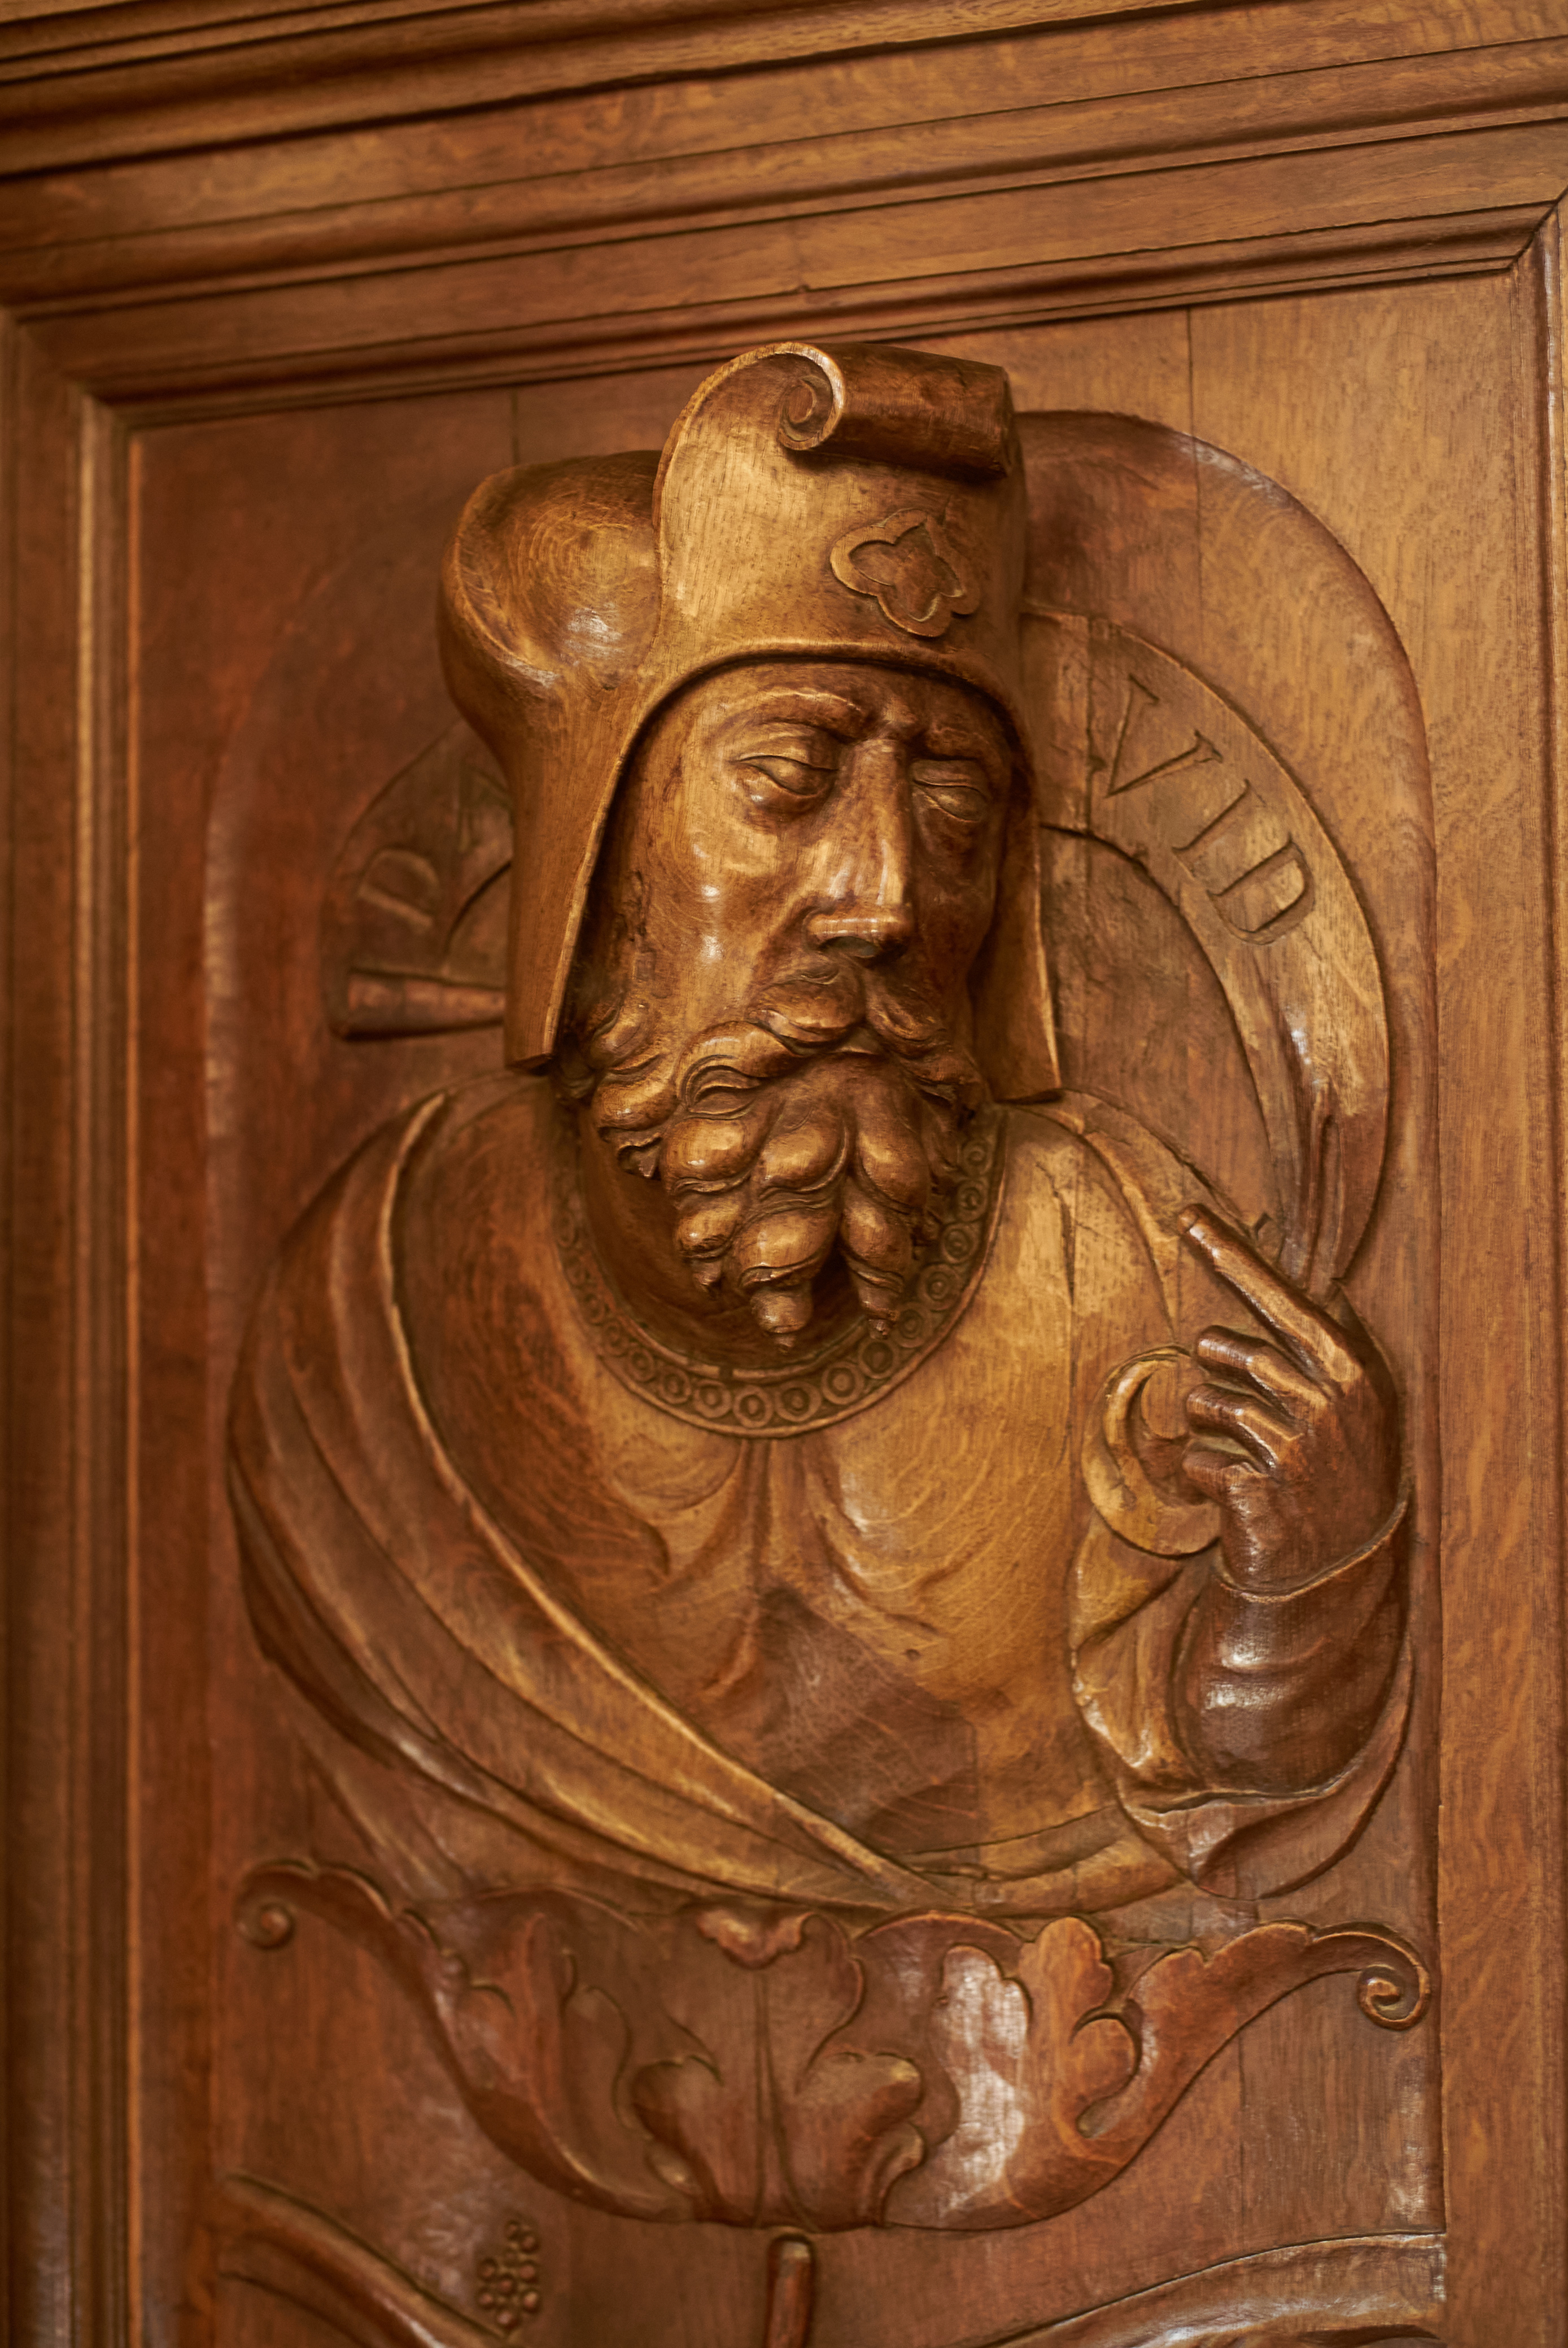
\includegraphics[height=\textheight]{photo_davidstalles_portrait.jpg}\thispagestyle{empty}
\restoregeometry

\end{document}